\documentclass[journal=jcisd8,manuscript=suppinfo]{achemso}

\usepackage{amsmath,amssymb}
\usepackage{graphicx}
\usepackage{booktabs}
\usepackage{multirow}
\usepackage{siunitx}
\usepackage[dvipsnames]{xcolor}

\title{Supporting Information: When Do Simple Models Win? Benchmarking Machine Learning for UV Absorption Prediction}

\author{Umesh Arampath}
\email{uarampath@mwbioprocessing.com}
\affiliation{Department of Mathematics, University of Iowa, Iowa City, USA}
\alsoaffiliation{Midwest Bioprocessing Center, Illinois, USA}

\author{Bryant Pero}
\affiliation{Midwest Bioprocessing Center, Illinois, USA}

\author{David Stewart}
\affiliation{Department of Mathematics, University of Iowa, Iowa City, USA}

\author{David Demirjian}
\affiliation{Midwest Bioprocessing Center, Illinois, USA}

\begin{document}

\section{Per-Fold Cross-Validation Results}
\label{sec:perfold}

Tables~\ref{tab:perfold_rf}--\ref{tab:perfold_chemberta} present per-fold results for all four model families on the primary Joung+Beard dataset (stratified 5-fold CV, 64/16/20 split).

\begin{table}[htbp]
\centering
\caption{Per-fold RF + Morgan FP results (tuned, with solvent).}
\label{tab:perfold_rf}
\begin{tabular}{ccccc}
\toprule
\textbf{Fold} & \textbf{RMSE (nm)} & \textbf{MAE (nm)} & $\boldsymbol{R^2}$ & \textbf{Pearson $r$} \\
\midrule
0 & 32.02 & 15.42 & 0.907 & 0.953 \\
1 & 30.74 & 14.79 & 0.918 & 0.959 \\
2 & 28.09 & 14.47 & 0.931 & 0.965 \\
3 & 32.58 & 15.56 & 0.908 & 0.953 \\
4 & 33.25 & 15.54 & 0.905 & 0.952 \\
\midrule
\textbf{Mean $\pm$ Std} & \textbf{31.34 $\pm$ 1.82} & \textbf{15.16 $\pm$ 0.44} & \textbf{0.914 $\pm$ 0.010} & \textbf{0.956 $\pm$ 0.005} \\
\bottomrule
\end{tabular}
\end{table}

\begin{table}[htbp]
\centering
\caption{Per-fold BiGRU + Solvent results (v2).}
\label{tab:perfold_bigru}
\begin{tabular}{ccccc}
\toprule
\textbf{Fold} & \textbf{RMSE (nm)} & \textbf{MAE (nm)} & $\boldsymbol{R^2}$ & \textbf{Pearson $r$} \\
\midrule
0 & 35.23 & 20.02 & 0.888 & 0.942 \\
1 & 37.33 & 20.86 & 0.879 & 0.937 \\
2 & 34.96 & 20.77 & 0.893 & 0.945 \\
3 & 37.62 & 21.51 & 0.877 & 0.937 \\
4 & 37.12 & 20.32 & 0.881 & 0.939 \\
\midrule
\textbf{Mean $\pm$ Std} & \textbf{36.45 $\pm$ 1.12} & \textbf{20.70 $\pm$ 0.51} & \textbf{0.884 $\pm$ 0.006} & \textbf{0.940 $\pm$ 0.003} \\
\bottomrule
\end{tabular}
\end{table}

\begin{table}[htbp]
\centering
\caption{Per-fold XGBoost + Morgan FP results (MSE loss, v2).}
\label{tab:perfold_xgboost}
\begin{tabular}{ccccc}
\toprule
\textbf{Fold} & \textbf{RMSE (nm)} & \textbf{MAE (nm)} & $\boldsymbol{R^2}$ & \textbf{Pearson $r$} \\
\midrule
0 & 34.55 & 20.15 & 0.892 & 0.945 \\
1 & 33.58 & 19.79 & 0.902 & 0.950 \\
2 & 30.63 & 19.31 & 0.918 & 0.959 \\
3 & 35.15 & 20.77 & 0.893 & 0.946 \\
4 & 34.58 & 20.23 & 0.897 & 0.948 \\
\midrule
\textbf{Mean $\pm$ Std} & \textbf{33.70 $\pm$ 1.61} & \textbf{20.05 $\pm$ 0.48} & \textbf{0.900 $\pm$ 0.009} & \textbf{0.950 $\pm$ 0.005} \\
\bottomrule
\end{tabular}
\end{table}

\begin{table}[htbp]
\centering
\caption{Per-fold ChemBERTa results (v2).}
\label{tab:perfold_chemberta}
\begin{tabular}{ccccc}
\toprule
\textbf{Fold} & \textbf{RMSE (nm)} & \textbf{MAE (nm)} & $\boldsymbol{R^2}$ & \textbf{Pearson $r$} \\
\midrule
0 & 49.31 & 23.88 & 0.780 & 0.899 \\
1 & 48.66 & 23.54 & 0.794 & 0.908 \\
2 & 47.70 & 23.05 & 0.801 & 0.909 \\
3 & 53.04 & 25.68 & 0.756 & 0.889 \\
4 & 53.24 & 25.39 & 0.756 & 0.890 \\
\midrule
\textbf{Mean $\pm$ Std} & \textbf{50.39 $\pm$ 2.30} & \textbf{24.31 $\pm$ 1.04} & \textbf{0.777 $\pm$ 0.019} & \textbf{0.899 $\pm$ 0.009} \\
\bottomrule
\end{tabular}
\end{table}


\section{Statistical Significance Tests}
\label{sec:significance}

Table~\ref{tab:significance} presents paired $t$-test results across the five cross-validation folds.
All model comparisons are statistically significant at $\alpha = 0.05$ using the parametric paired $t$-test.
With only $n = 5$ folds, the Wilcoxon signed-rank test (a non-parametric alternative) yields $p = 0.0625$ for all comparisons (the minimum achievable $p$-value when all 5 paired differences are concordant), providing strong directional evidence despite not reaching conventional significance.

\begin{table}[htbp]
\centering
\caption{Paired $t$-test results for RMSE comparisons across 5 folds.}
\label{tab:significance}
\begin{tabular}{lccc}
\toprule
\textbf{Comparison} & $\boldsymbol{t}$ & $\boldsymbol{p}$ & \textbf{Significant?} \\
\midrule
RF vs.\ BiGRU              & $-7.08$ & 0.002 & Yes \\
RF vs.\ XGBoost            & $-8.94$ & 0.001 & Yes \\
RF vs.\ ChemBERTa          & $-31.0$ & $<$0.001 & Yes \\
XGBoost vs.\ BiGRU         & $-4.38$ & 0.012 & Yes \\
XGBoost vs.\ ChemBERTa     & $-21.8$ & $<$0.001 & Yes \\
BiGRU vs.\ ChemBERTa       & $-16.0$ & $<$0.001 & Yes \\
RF: solvent vs.\ no-solvent  & $-11.46$ & $<$0.001 & Yes \\
BiGRU: solvent vs.\ no-solvent & $-3.90$ & 0.018 & Yes \\
\bottomrule
\end{tabular}
\end{table}


\section{RF Hyperparameter Sensitivity}
\label{sec:rf_tuning}

The RF hyperparameter grid search evaluated 432 configurations varying the number of trees ($B \in \{100, 500, 1000\}$), maximum features per split ($\sqrt{d}$, $0.1d$, $0.3d$), maximum tree depth (None, 30, 50), minimum samples per leaf (1, 2, 5), fingerprint radius (2, 3), and fingerprint length (1024, 2048).
The search was conducted on fold~0 using the validation set for model selection.

The most influential parameter was \texttt{max\_features}: all top-10 configurations used $0.3d$ (30\% of features per split), compared to the scikit-learn default of $\sqrt{d}$ ($\approx$1.6\% of 4096 features).
This finding suggests that Morgan fingerprint features are sufficiently decorrelated that broader feature sampling per split improves performance.
The number of trees ($B$) showed diminishing returns beyond 500, and maximum depth had negligible effect (unlimited depth was optimal), indicating that the dataset does not suffer from overfitting with deep trees.


\section{BiGRU Training Curves}
\label{sec:learning_curves}

Figure~\ref{fig:learning_curves} shows the training and validation MAE curves for the BiGRU models, averaged across folds with $\pm 1$ standard deviation bands.
Both models converge within 75--125 epochs, with early stopping preventing overfitting.
The gap between training and validation curves indicates mild overfitting, consistent with the relatively small dataset size (12K training samples per fold).

\begin{figure}[htbp]
    \centering
    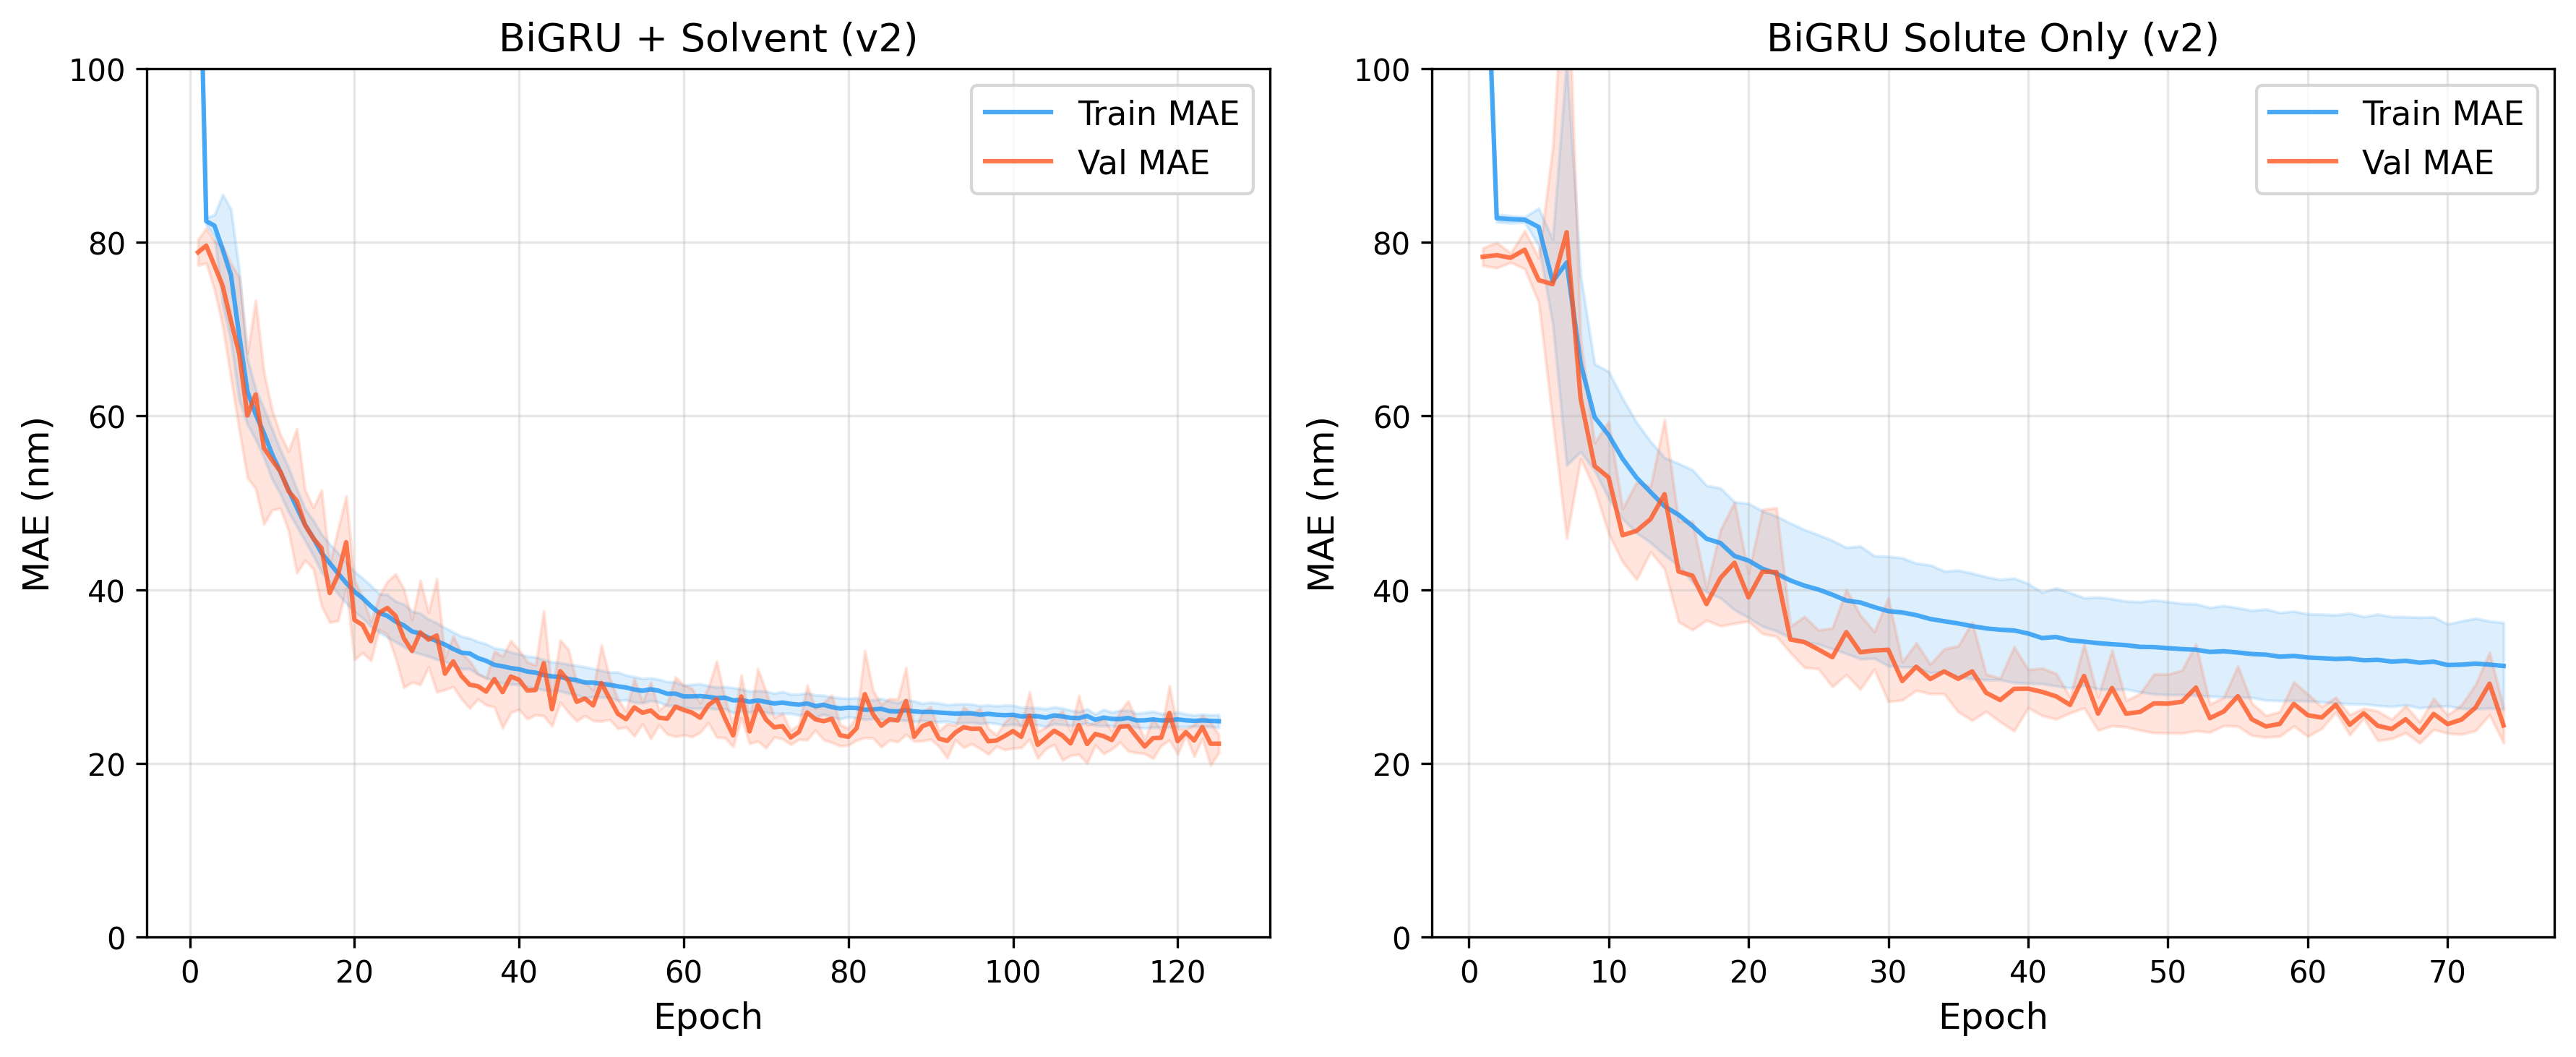
\includegraphics[width=0.9\textwidth]{results/learning_curves.png}
    \caption{BiGRU training curves showing training and validation MAE vs.\ epoch, averaged across folds. Shaded regions denote $\pm 1$ standard deviation. Left: BiGRU with solvent encoding. Right: BiGRU with solute only.}
    \label{fig:learning_curves}
\end{figure}


\section{ChemBERTa Learning Curves}
\label{sec:chemberta_curves}

Figure~\ref{fig:chemberta_curves} shows the ChemBERTa training and validation MAE curves across all five folds.
All folds converge within 40--60 epochs, with the final validation MAE plateauing around 24--26~nm.
The gap between training and validation MAE is larger than for BiGRU, consistent with ChemBERTa's 44.1M parameters being overparameterized for the $\sim$12K training samples available per fold.

\begin{figure}[htbp]
    \centering
    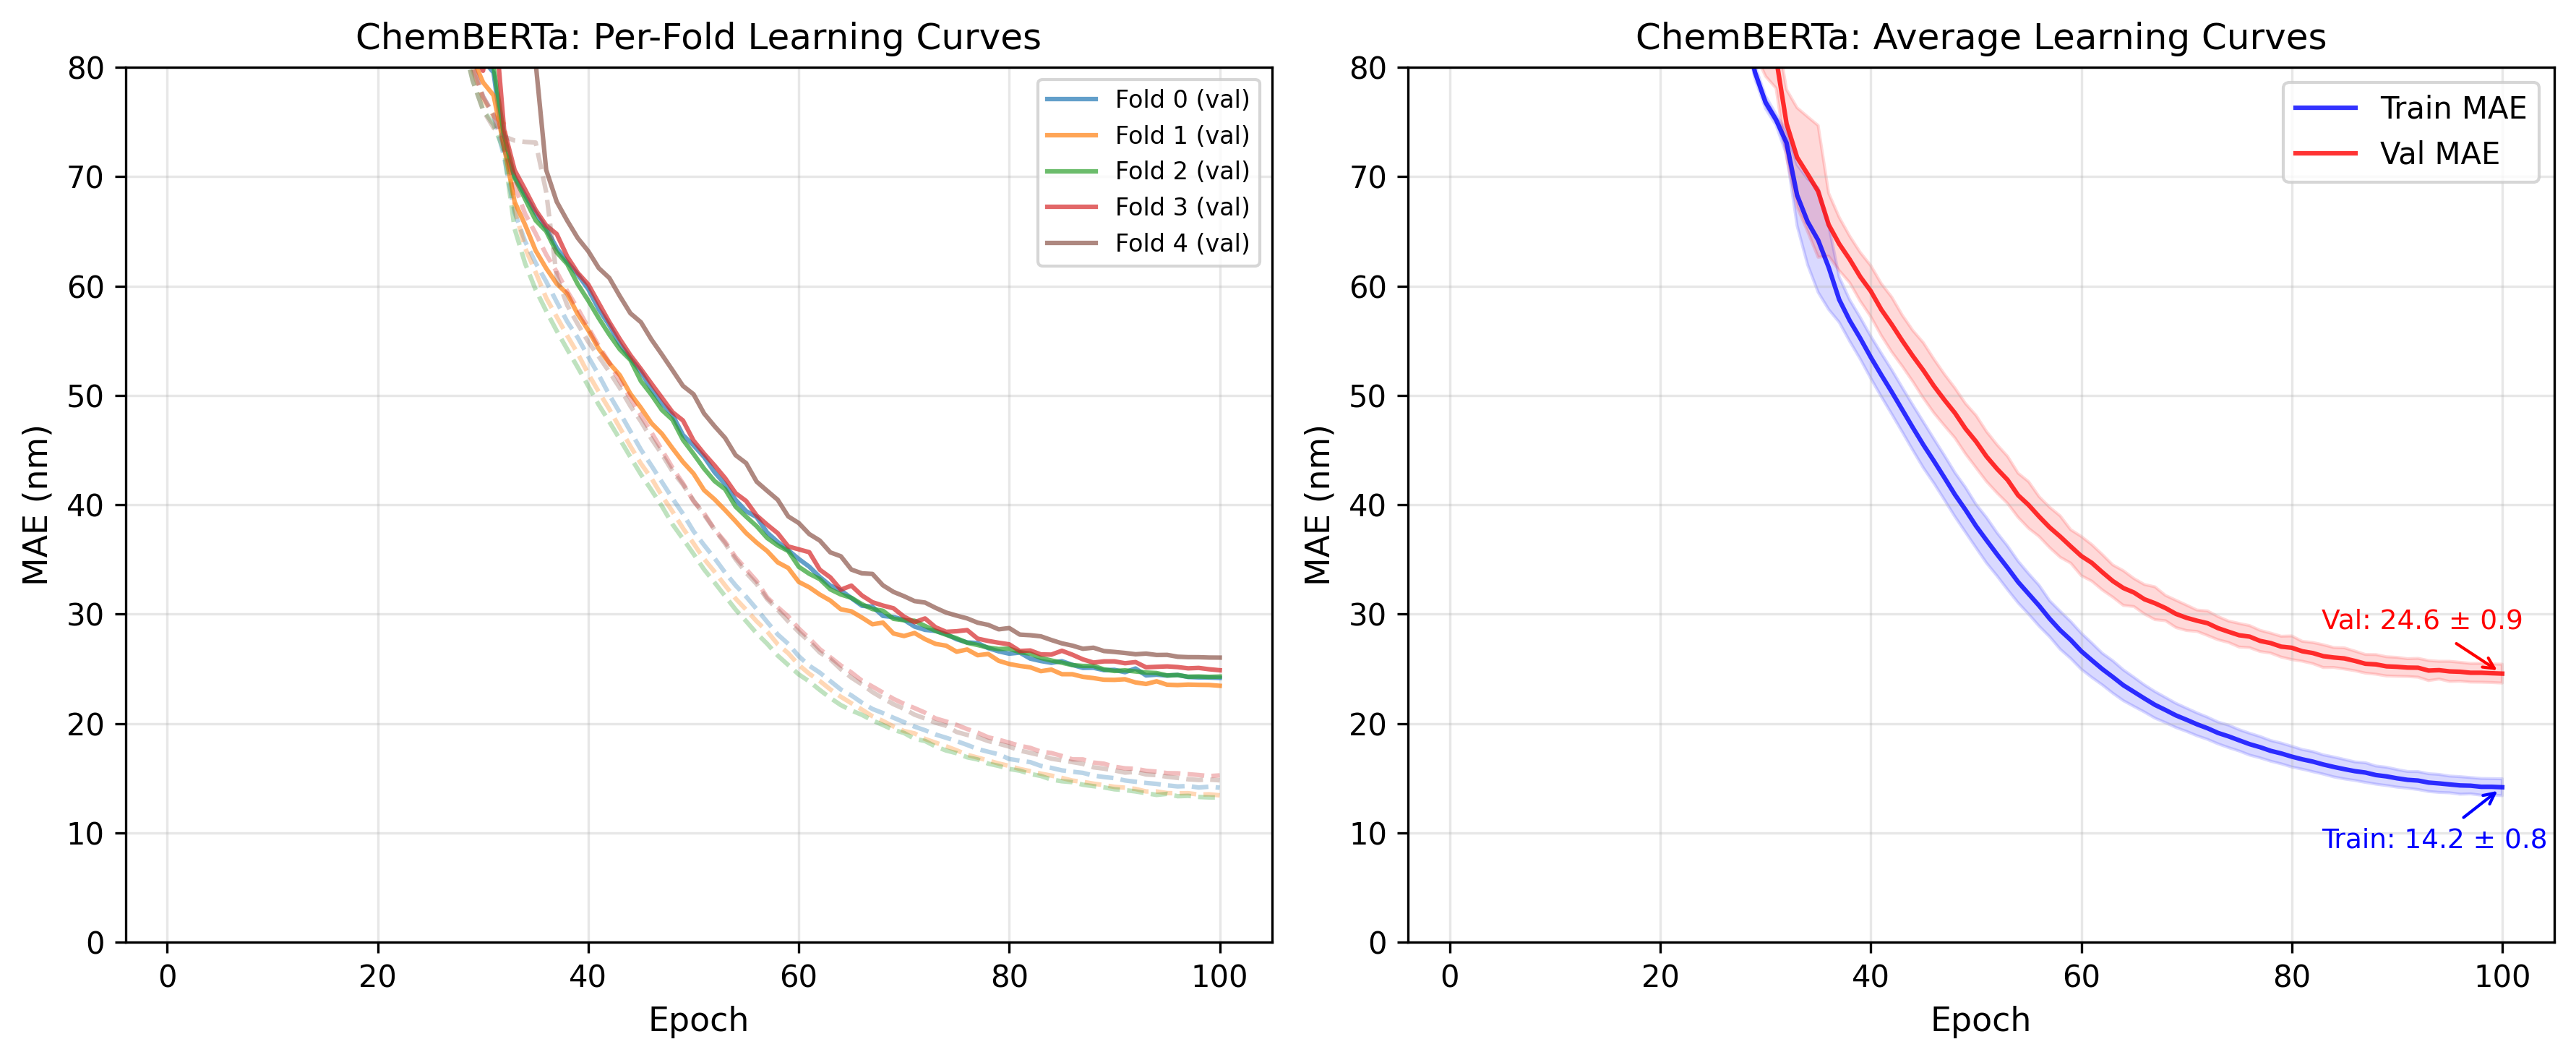
\includegraphics[width=\textwidth]{results/chemberta_learning_curves.png}
    \caption{ChemBERTa fine-tuning learning curves. Left: per-fold validation MAE (solid) and training MAE (dashed). Right: mean $\pm$ 1 standard deviation across folds, with final values annotated.}
    \label{fig:chemberta_curves}
\end{figure}


\section{Hyperparameter Tuning Asymmetry}
\label{sec:tuning_asymmetry}

Table~\ref{tab:tuning_asymmetry} compares the effect of hyperparameter tuning for both RF and BiGRU, demonstrating that the in-distribution performance gap between model families is not an artifact of asymmetric tuning effort.

\begin{table}[htbp]
\centering
\caption{Effect of hyperparameter tuning on cross-validated performance (stratified 5-fold CV).}
\label{tab:tuning_asymmetry}
\begin{tabular}{lccc}
\toprule
\textbf{Model} & \textbf{RMSE (nm)} & \textbf{MAE (nm)} & \textbf{Improvement} \\
\midrule
RF (default, $\sqrt{d}$)         & 32.18 $\pm$ 1.74 & 15.42 $\pm$ 0.44 & --- \\
RF (tuned, $0.3d$)               & 31.34 $\pm$ 1.82 & 15.16 $\pm$ 0.44 & $-$2.6\% RMSE \\
\midrule
BiGRU (default, 2L/128u)         & 36.45 $\pm$ 1.12 & 20.70 $\pm$ 0.51 & --- \\
BiGRU (tuned, 3L/256u)\textsuperscript{$\dagger$} & 33.33\textsuperscript{$\dagger$} & --- & $-$8.6\% RMSE \\
\bottomrule
\end{tabular}
\smallskip

\textsuperscript{$\dagger$}Fold~0 validation RMSE from HPO (25 Optuna trials); full 5-fold CV pending.
\end{table}

BiGRU HPO was conducted using Optuna TPE (25 trials on fold~0), yielding an 8.6\% RMSE improvement over the default architecture.
Even the default RF (RMSE = 32.18~nm) outperforms the default BiGRU (RMSE = 36.45~nm) by 12\%, while RF tuning provides only an additional 2.6\% improvement.
BiGRU tuning narrows this gap substantially, but the remaining difference suggests that the fingerprint representation has an inherent advantage for in-distribution UV absorption prediction.
ChemBERTa hyperparameters were not tuned due to the prohibitive training cost ($\sim$3 hours per fold for 44.1M parameters).


\section{BiGRU Character-Type Saliency}
\label{sec:chartype_saliency}

Figure~\ref{fig:bigru_chartype} shows the mean gradient saliency aggregated by SMILES character type across all wetlab validation molecules.
Bond symbols (\texttt{=}, \texttt{\#}) receive the highest mean saliency, reflecting the critical role of double and triple bonds in establishing conjugated $\pi$-systems that determine UV absorption.
Heteroatoms (N, O, S) rank second, consistent with their role as electron donors and acceptors in chromophores, while aromatic atom characters and aliphatic carbons receive lower saliency, and brackets/syntax characters contribute minimally.

\begin{figure}[htbp]
    \centering
    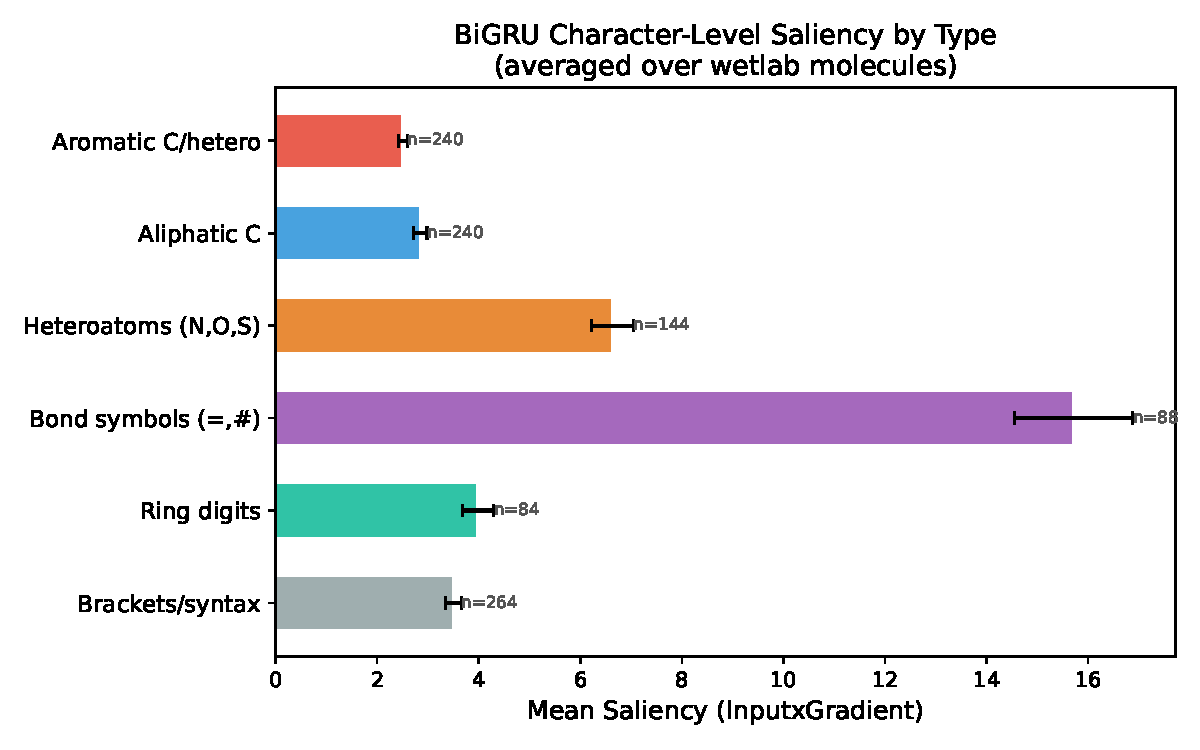
\includegraphics[width=0.65\textwidth]{results/bigru_saliency_chartype.pdf}
    \caption{Mean BiGRU gradient saliency by SMILES character type, averaged over all wetlab validation molecules. Bond symbols (\texttt{=}, \texttt{\#}) and heteroatoms receive the highest saliency, consistent with the role of conjugated $\pi$-systems and electron-donating/withdrawing groups in determining UV absorption.}
    \label{fig:bigru_chartype}
\end{figure}

\end{document}
